\section{Einfluss äußerer Störfaktoren auf die Basisstation}

Um eine Einschätzung dafür zu bekommen, wie sehr das Magnetfeld an der Basisstation von äußeren Störfaktoren, wie zum Beispiel der Hütte, abhängig war, wurde ein Profil von der Basisstation aus an der Hütte vorbei gelegt. Das zugehörige Messprotokoll befindet sich im Anhang in Abbildung \ref{fig:MPHuette}.

In Diagramm \ref{fig:plot_huette} sind die Messergebnisse graphisch dargestellt. Es ist zu erkennen, dass das Magnetfeld bei 19\,m, also neben der Hütte, abnimmt. In der Nähe der Basisstation wird der Messwert jedoch wieder annähernd konstant. Um jedoch sicher sagen zu können, dass der Einfluss der Hütte nur bis zu einer Entfernung von 5\,m zu messen ist, hätten wir die Messung auf der anderen Seite der Basisstation noch weiter führen müssen.

\begin{figure}[h!]
 \centering
 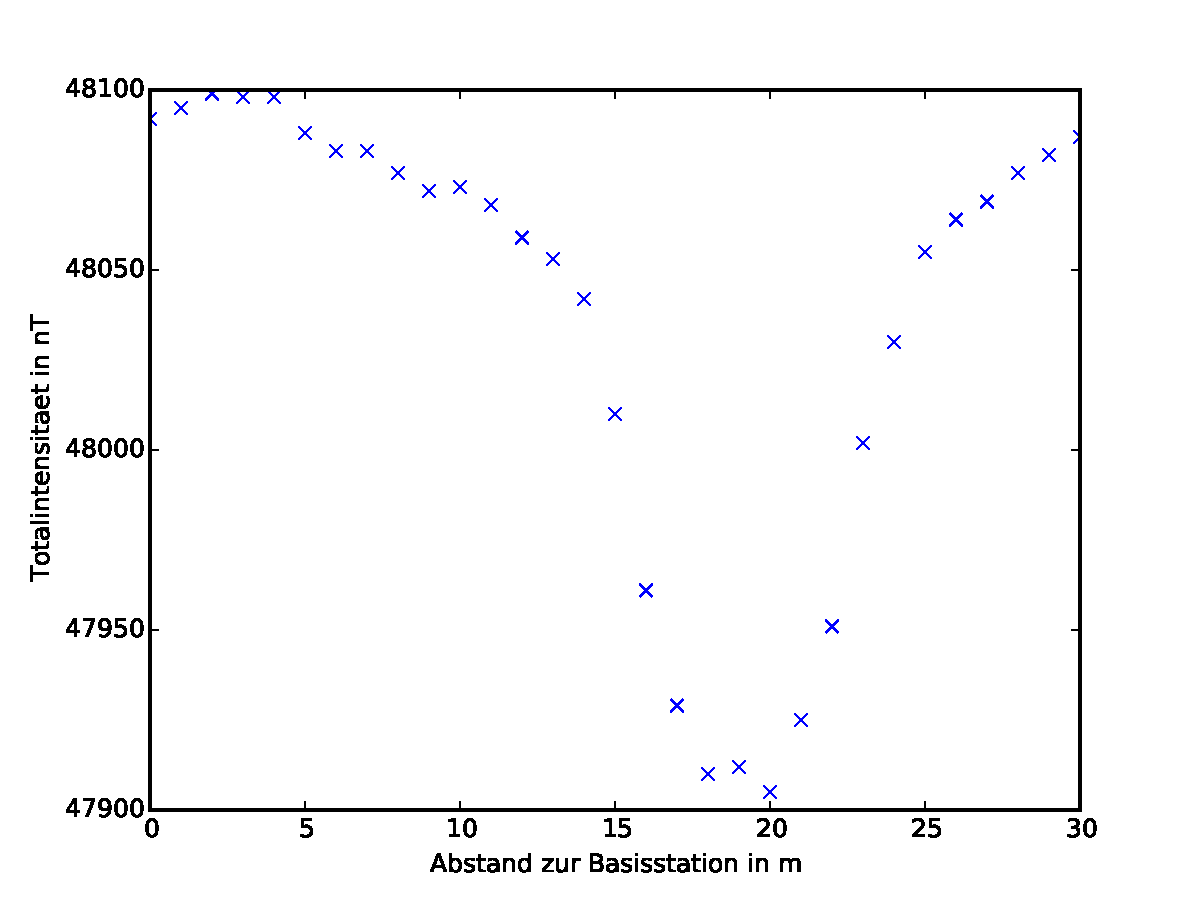
\includegraphics[width=\textwidth]{fig/plot_huette.pdf}
 \caption[Einfluss der Umgebung auf die Basismessung]{Einfluss der Umgebung auf die Basismessung. Die Totalintensität in nT ist über dem Abstand zur Basisstation in m aufgetragen. Der Tisch mit vielen Arbeitsmaterialien befindet sich bei 13,5\,m und die Hütte bei 19\,m.}
 \label{fig:plot_huette}
\end{figure}

% \begin{figure}[h!]
%  \centering
%  \includegraphics[width=\textwidth]{fig/Messprotokolle/}
%  \caption{}
%  \label{fig:}
% \end{figure}

\section{Einfluss eines vorbeifahrenden Traktors}

Es fuhr an diesem Tag mehrmals ein kleiner Traktor an der Messwiese vorbei. Um seinen Einfluss auf das lokale Magnetfels zu untersuchen, wurde während einer Vorbeifahrt eine Messung mit dem Gradiometer durchgeführt. Dieses wurde in einem Abstand von circa einem Meter neben dem Feldweg möglichst still gehalten. Das Diagramm dieser Messung ist in Abbildung \ref{fig:plot_traktor} zu sehen.

\begin{figure}[h!]
 \centering
 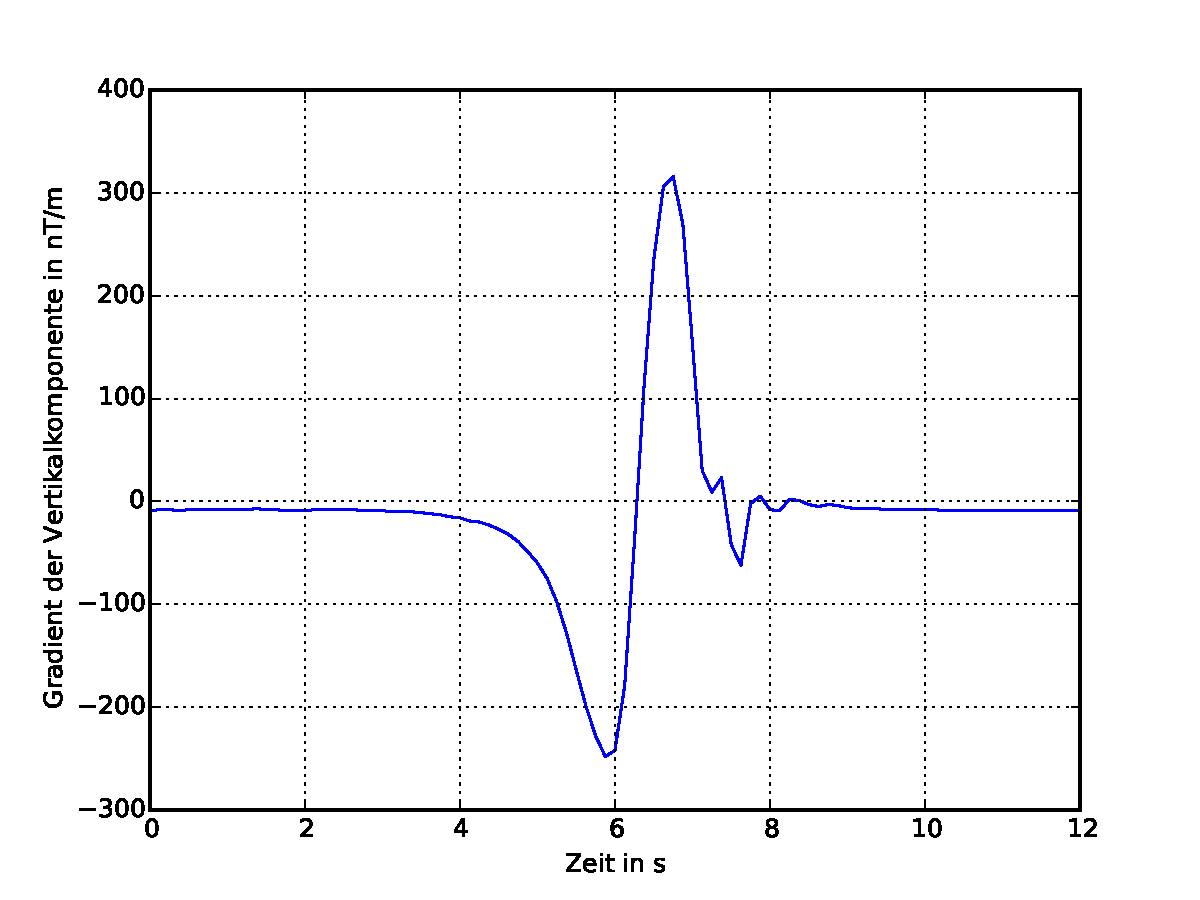
\includegraphics[width=\textwidth]{fig/traktor_ausschnitt.pdf}
 \caption[Messung während einer Vorbeifahrt des Traktors]{Messung während einer Vorbeifahrt des Traktors. Der Gradient der Vertikalkomponente ist über der Zeit nach Beginn der Messung aufgetragen. Es wurde 30\,s lang gemessen. Da der Einfluss nur bis zu Sekunde 9 zu sehen ist, ist hier nur der entsprechende Ausschnitt gezeigt.}
 \label{fig:plot_traktor}
\end{figure}

Zur Zeit der Peaks war der Traktor dem Gradiometer am nächsten. Es ist also deutlich zu erkennen, dass der Traktor einen Einfluss auf das Magnetfeld seiner Umgebung hat. Es ist außerdem zu erkennen, dass der Einfluss sechs Sekunden lang in Form mehrerer Ausschläge zu messen war. Unter der Annahme, dass dieser mit einer Geschwindigkeit von $\eb{20}{km}{h}\approx\eb{5,6}{m}{s}$ fuhr, ist sein Einfluss mit dem Gradiometer also in einer Distanz von $\eb{5,6}{m}{s}\cdot\e{3}{s}\approx\e{16,7}{m}$ noch zu messen. Damit ist sein Einfluss größer als erwartet und es hätte noch genauer darauf geachtet werden müssen, nicht bei einer Vorbeifahrt zu messen.